\documentclass{article}

% Language setting
% Replace `english' with e.g. `spanish' to change the document language
\usepackage[english]{babel}
\usepackage{geometry}
\usepackage{algorithm}
\usepackage[noend]{algpseudocode}

% Set page size and margins
% Replace `letterpaper' with `a4paper' for UK/EU standard size
 \geometry{
 a4paper,
 total={170mm,257mm},
 left=20mm,
 top=20mm,
 }
% Useful packages
\usepackage{amsmath}
\usepackage{amssymb}

\usepackage{graphicx}
\usepackage[colorlinks=true, allcolors=blue]{hyperref}



\title{Reasoning and Agents}
\author{Finlay Ross-Davie}
\date{17th January 2024}

\begin{document}
\maketitle


\section{Intelligent Agents}

\subsection{Definition of agents and environments}

An \textbf{Agent} is anything that can be viewed as perceiving its environment through \textbf{sensors} and acting upon that environment through \textbf{actuators} \newline. 

\textbf{Percept} is a term used to refer to the agent's perceptual inputs at any given instant. An agent's 

\textbf{percept sequence} is the complete history of everything the agent has ever perceived \newline

An agent's choice of action at any given instant can depend on the entire percept sequence observed, but not anything it hasn't perceived.

An agent's behavior is described, mathematically speaking, by the \textbf{agent function} that maps any given percept sequence to an action.

The agent function for an artificial agent will be implemented by an \textbf{agent program}.

i.e, The agent program is an abstract mathematical description; the agent program is a concrete implementation, running within some physical system 

\subsection{The Concept of rationality}

A \textbf{performance measure} evaluates any given sequence of environment states to capture whether the agent has performed well.

In general, it is better to design performance measures according too what one actually wants in the environment, rather than according to how one thinks the agent should behave. \newline

What is rational at any given time depends on four things:

\begin{itemize}
    \item The performance measure that is defined the criterion of success
    \item The agents prior knowledge of the environment
    \item The actions that the agent can perform
    \item The agent's percept sequence to date.

\end{itemize}

The definition of a \textbf{rational agent}:

For each possible percept sequence, a rational agent should select an action that is expected to maximize its performance measure, given the evidence provided by the percept sequence and whatever built in knowledge the agent has. \newline

An \textbf{omniscient} agent knows the actual outcome of its actions and can act accordingly; but omniscience is impossible in reality.

Rationality maximises expected performance

To the extent that an agent relies on the prior knowledge of its designer rather than on its own percepts, we can say that the agent lacks \textbf{autonomy}. A rational agent should be autonomous - it should learn what it can to compensate for a partial or incorrect prior knowledge

The \textbf{task environment} is made up of  the performance measure, the environment, and the agent's actuators and sensors. This is also referred to as the \textbf{PEAS} (Performance, Environment, Actuators, Sensors) description \newline

If an agent's sensors give it access to the complete state of the environment at each point in time, then one can say that the task environment is \textbf{Fully observable}. A task environment is effectively fully observable if the sensors detect all aspects that are relevant to the choice of action; relevance, in turn depends on the performance measure. An environment might be \textbf{partially observable} because of noisy and inaccurate sensors or because parts of the state are simply missing from the sensor data \newline

If the next state of the environment is completely determined by the current state and the action executed by the agent, the environment is \textbf{deterministic}; otherwise it is \textbf{stochastic}. \newline

In an \textbf{episodic} task environment, the agent's experience is divided into atomic episodes. In each episode the agent receives a percept and then performs a single action. The next action does not depend on the actions taken in previous episodes. In \textbf{sequential} environments, the current decision could affect all future decisions. \newline 

If the environment can change while an agent is deliberating then the environment is \textbf{dynamic} for that agent, otherwise it is \textbf{static}. \newline

In a \textbf{known} environment, the outcomes (or outcome probabilities if the environment is stochastic) for all actions are given. If an environment is \textbf{unknown} the agent will have to learn how it works in order for it to make good decisions.

\subsection{The structure of agents}

agent = architecture + program

Where \textbf{architecture} is some sort of computing device with physical sensors and actuators.

Agent programs simply take the current percept as input from the sensors and return an action to the actuators. If the agent's actions need to depend on the entire percept sequence, the agent will hve to remember the percepts.

One kind of agent is the \textbf{simple reflex agent}. These agents select actions on the basis of the current percept, ignoring the rest of percept history. \

A \textbf{model} is a description of how the next state depends on the current state and action. A \textbf{model-based agent} is an agent that uses a model to keep track of the current state of the world, then chooses an action in the same way as the reflex agent. \newline

\textbf{Goal} information describes situations that are desirable. For \textbf{Goal based agents} the agent combine program will combine this goal information with the model to choose actions that achieve the goal. \newline

Goals alone are not enough to generate high-quality behaviour in most environments. An agent's \textbf{utility function} is essentially an internalization of the performance measure. If the internal utility function and the external performance measure are in agreement, then an agent that chooses actions to maximise its utility will be rational according to the external performance measure. A rational \textbf{utility-based} agent chooses the action that maximises the expected utility of the action outcomes. \newline

All agents can improve their performance through \textbf{learning}. A \textbf{learning agent} can be divided into four conceptual components:
\begin{itemize}
    \item Critic - Provides feedback to learning element
    \item Learning element - Responsible for making improvements
    \item Problem generator - Responsible for suggesting actions that will lead to new and informative experiences
    \item Performance element - Responsible for selecting external actions
\end{itemize}

\section{Search Problems}

A search strategy is defined by picking the order of node expansion
Nodes are taken from the frontier. 

\subsection{Uninformed search}



\textbf{Uninformed search} strategies have no additional information about states beyond that provided in the problem definition. 

A search algorithm is \textbf{complete} if it always finds a solution when one exists. A search algorithm is \textbf{optimal} if any found solution is optimal (has lowest possible cost).


\subsubsection{Breadth-first search}

Breadth-first search is a strategy in which all the nodes are expanded at a given depth in the search tree before any nodes at the next level are expanded. 

This is implemented by using a FIFO queue for the frontier. This leads to new nodes going to the back of the queue, and old nodes, getting expanded first. 

This search strategy:
\begin{itemize}
    \item Is \textbf{Complete} is b is finite
    \item Has \textbf{time complexity} of $b+b^2+b^3 \ldots +b^d = O(b^d)$ in the worst case
    \item Has \textbf{space complexity} of $O(b^d)$ since it keeps every node in memory
    \item Is \textbf{Optimal} if cost = 1 per step
\end{itemize}

\subsubsection{Depth-first search}

Depth-first search is a strategy in which the deepest unexpanded node is expanded. 
This is implemented using a LIFO queue. This leads to new successors going at the front. 

This search strategy:
\begin{itemize}
    \item Is \textbf{not complete} since it fails in infinite-depth and spaces with loops
    \item Has \textbf{time complexity} of $O(b^m)$ 
    \item Has \textbf{space complexity} of $O(bm)$ linear since explored nodes with no descendants in the frontier are removed from memory
    \item Is \textbf{not optimal}
\end{itemize}

\textbf{Depth-limited} search is a implementation with a depth limit l, i.e., nodes at depth l have no successors

This search strategy:
\begin{itemize}
    \item Is \textbf{not complete} 
    \item Has \textbf{time complexity} of $O(b^l)$ 
    \item Has \textbf{space complexity} of $O(bl)$ linear since explored nodes with no descendants in the frontier are removed from memory
    \item Is \textbf{not optimal}
\end{itemize}

\subsubsection{Iterative deepening search}

Iterative deepening search is a strategy used in combination with depth-first search, that finds the best depth limit. It gradually increases the limit (0, 1,..) until a goal is found. This will occur when the depth limit reaches d, the depth of the shallowest goal node. . 

This search strategy:
\begin{itemize}
    \item Is \textbf{complete} 
    \item Has \textbf{time complexity} of $O(b^d)$ 
    \item Has \textbf{space complexity} of $O(bd)$
    \item Is \textbf{optimal} if step cost is 1
\end{itemize}

\subsection{Informed Search}

An informed search strategy is one that uses problem-specific knowledge beyond the definition of the problem itself.

\textbf{Best-first search} is an instance of the general TREE-SEARCH or GRAPH SEARCH algorithm. In best-first search a node is selected for expansion based on an \textbf{evaluation function}, $f(n)$, the evaluation function is construed as a cost estimate so the node with the lowest evaluation is expanded first. 
Most best-first algorithms include a \textbf{heuristic function}, $h(b)$. $h(n)$ estimates the cost of the cheapest path from state at node n to a goal state.  

A heuristic $h(n)$ is \textbf{admissible} if for every node n: $$h(n) \leq h^*(n)$$ where $h^*(n)$ is the true cost to reach the goal state from n 

An admissible heuristic never overestimates the cost to reach the goal i.e., it is optimistic. 

A heuristic $h(n)$ is \textbf{consistent}, if its estimate is always less than or equal to the estimated distance from any neighbouring vertex to the goal, plus the cost of reaching that neighbor .Formally: if for every node n, every successor n' of n generated by any action a: $$h(n) \leq c(n, a, n') + h(n')$$ 


\subsubsection{Greedy best-first search}

Greedy best-first search tries to expand the node that is closest to the goal.

The evaluation function is simply the heuristic $$f(n) = h(n)$$

This search strategy:
\begin{itemize}
    \item Is \textbf{not complete} since it can get stuck in loops
    \item Has \textbf{time complexity} of $O(b^m)$ 
    \item Has \textbf{space complexity} of $O(b^m)$ since it keeps all nodes in memory
    \item Is \textbf{not optimal}
\end{itemize}

\subsubsection{A* Search}

A* search evaluates nodes by combining $g(n)$, the cost to reach the node, and $h(n)$, the cost to get from the node to the goal.

The evaluation function is given as $$f(n) = g(n) + h(n)$$

If $h(n)$ is admissible, A* using TREE-SEARCH is optimal

If $h(n)$ is consistent, A* using GRAPH-SEARCH is optimal \newline

This search strategy:
\begin{itemize}
    \item Is \textbf{Complete} unless there are infinitely many nodes with $f \leq f(G)$
    \item Has exponential \textbf{time complexity}
    \item Keeps all nodes in memory
    \item Is \textbf{optimal}
\end{itemize}

\subsection{Smart Search using constraints}

A \textbf{constraint satisfaction problem} consists of a set of \textbf{variables} X = ${X_1,\ldots,X_n}$, a set of \textbf{domains},$D = {D_1,\ldots,D_n}$ where each domain $D_i$ is a set of possible values for variable $X_i$ and a set of \textbf{constraints} C that specify acceptable combinations of values where each $c \in C$ consists of a \textbf{scope}, tuple of variables involved in the constraint and a \textbf{relation} that defines the values that the variables can take.

Varieties of constrains:
\begin{itemize}
    \item \textbf{Unary} constraints involve a single variable
    \item \textbf{Binary} constraints involve pairs of variables
    \item \textbf{Higher-order} constraints involve 3 or more variables
    \item \textbf{Global} constraints involve an arbitrary number of variables
\end{itemize}

A variable in a CSP is \textbf{arc-consistent} if every value in its domain satisfies the variables binary constraints. 
More formally, $X_i$ is arc-consistent with respect to another variable $X_j$ if for every value in the current domain $D_i$ there is some value in the domain $D_j$ that satisfies the binary constraint on the arc $(X_i,X_j)$

All CSPs are \textbf{commutative}. A problem is commutative if the order of application of any given set of actions has no effect on the outcome. When assigning values to variables in CSPs, we reach the same partial assignment regardless of order. We only need to consider assignments to a single variable at each node

\subsubsection{Backtracking search}

The term \textbf{backtracking search} is used for a depth-first search that chooses values for one variable at a time and backtracks when a variable has no legal values left to assign.

In simple terms backtracking works by choosing a variable, assigning a value to it, and then recursively trying to solve the rest of the problem.

\begin{algorithm}
\begin{algorithmic}

\Procedure{BacktrackingSearch}{$csp$}
    \Comment{returns a solution or failure}
    \State return Backtrack($[],csp$)
\EndProcedure

\Procedure{Backtrack}{$(assignment,csp)$}

\If{$assignment$ is complete}
    \State return $assignment$
\EndIf
\State $var \leftarrow$ SELECT-UNASSIGNED-VARIABLE$(csp)$
\For{\State each value in ORDER-DOMAIN-VALUES($var,assignment,csp$)}

    \If{$value$ is consistent with $assignment$}
        \State add {$var = value$} to $assignment$
        \State $inferences \leftarrow$ INFERENCE($csp,var,value$)
        \If{$inferences \neq failure$}
            \State add $inferences$ to $assignment$
            \State $result \leftarrow $ BACKTRACK($assignment,csp$)
                    \If{$result \neq failure$}
                        \State return result
                    \EndIf
                \EndIf
            \EndIf
    \State return $result$

\EndFor

\State return $failure$

\EndProcedure

\end{algorithmic}
\end{algorithm}

Variable ordering in backtracking-search (SELECT-UNASSIGNED-VARIABLE) can be decided in various manners to garner gains in speed. The \textbf{most constrained variable} technique chooses the variable with the fewest legal values, this reduces branching. \newline

Value ordering (ORDER-DOMAIN-VALUES)can be done using various techniques such as \textbf{least constraining value} which chooses the value that rules out the fewest values in the remaining variables for a given variable. \newline 

Inference (INFERENCE) allows one to potentially detect inevitable failure early. For example, \textbf{forward checking} keeps track of remaining legal values for unassigned variables and terminates the search when any variable has no legal values. Another form of inference, \textbf{constraint propagation} repeatedly enforces constrains locally . \newline 

The pair $(X,Y)$ of constraint variables is \textbf{arc consistent} if for each value $x \in D_X$ there exists a value $y \in D_Y$ such that the assignments $X=x$ and $Y=y$ satisfy all binary constraints between $X$ and $Y$. A CSP is arc consistent if all variable pairs are arc consistent. \newline

The most popular algorithm to make every variable arc-consistent is called AC-3 which maintains a queue of arcs to consider. Initially, the queue contains all the arcs in the CSP. AC-3 then pops off an arbitrary arc $(X_i,X_j)$ from the queue and makes $X_i$ arc-consistent with respect to $X_j$. If this leaves $D_i$ unchanged, the algorithm just moves on to the next arc. If this makes $D_i$ smaller, then all arc $(X_k,X_i)$ where $X_k$ is a neighbor of $X_i$ are added to the queue since the change in $D_i$ might enable further reductions in the domains of $D_k$. If $D_i$ is revised down to nothing, the CSP has no consistent solution and AC-3 can return failure


\begin{algorithm}
\begin{algorithmic}

\Procedure{AC-3}{$csp$}
    \Comment{returns false if an inconsistency is found and true otherwise}
    \While{queue is not empty}
        \State $(X_i,X_j) \leftarrow$ REMOVE-FIRST(queue)
        \If{REVISE($csp,X_i,X_j$)} 
            \If{size of $D_i = 0$}
                \State \textbf{return} false
                \For{each $X_k$ in $X_i.$NEIGHBORS - ${x_J}$}
                    \State add $(X_k,X_i)$ to queue
                \EndFor
            \EndIf
        \EndIf
    \EndWhile 
    \State \textbf{return} true 
\EndProcedure

\Procedure{REVISE}{$(csp, X_i,X_j)$}

    \State $revised \leftarrow false$
    \For{each $x$ in $D_i$}
        \If{no value $y$ in $D_j$ allows $(x,y)$ to satisfy the constraint between $X_i$ and $X_j$}
            \State delete $x$ from $D_i$
            \State $revised \leftarrow true$
        \EndIf
        
    \EndFor

    \State return $revised$

\EndProcedure

\end{algorithmic}
\end{algorithm}

For REMOVE-FIRST or SELECT-UNASSIGNED-VARIABLE in the AC-3 and back-tracking search algorithms we may use a heurstic such as \textbf{minimum remaining values}, this chooses the variable that is most likely to cause a failure soon.  

\section{Adversarial Search}

\textbf{Zero-sum games} are deterministic, turn-taking and only have two players. Utilities at the end of a zero-sum game are equal and opposite (summing to 0). 

\textbf{Pruning} allows us to ignore portions of the search tree that make no difference to the final choice.
\subsubsection{Minimax}

A minimax game can be formally defined as being a kind of search problem with the following elements
\begin{itemize}
    \item $S_0:$ The initial state
    \item PLAYER(s): Define which player has the move in a state (MAX or MIN)
    \item ACTIONS(s): Returns the set of legal moves in a state
    \item RESULT(s,a): The transition model, which defines the result of a move
    \item TERMINAL-TEST(s): A terminal test, which is true when the game is over and false otherwise
    \item UTILITY(s,p): A utility function defines the numeric value for a game that ends in terminal state $s$ for a player $p$
\end{itemize}

The minimax value of a node is the utility for MAX of being in corresponding state

\begin{equation}
MINIMAX(s) =
    \begin{cases}
        UTILITY(S) & \text{if TERMINAL-TEST(s)} \\
        max_{a \in Actions(s)}MINIMAX(RESULT(s,a)) & \text{if} PLAYER(s) = MAX \\
        min_{a \in Actions(s)}MINIMAX(RESULT(s,a)) & \text{if} PLAYER(s) = MIN \\
            
    \end{cases}
\end{equation}

\begin{algorithm}
\begin{algorithmic}

\Procedure{MINIMAX-DECISION}{state}
    \State \textbf{return} $argmax_{a \in ACTIONS_{(s)}}MIN-VALUE(RESULT(state,a))$
\EndProcedure \newline

\Procedure{MAX-VALUE}{$state$}
    \Comment{returns a utility value}
    \If{TERMINAL-TEST(state)}
        \State \textbf{return} UTILITY(state)
    \EndIf
    \State $v \leftarrow -\infty$
    \For{each a in ACTIONS(state)}
        $v \leftarrow MAX(v,MIN-VALUE(RESULT(s,a)))$
    \EndFor

    \State \textbf{return} $v$ 
\EndProcedure \newline

\Procedure{MIN-Value}{$state)$}
    \If{TERMINAL-TEST(state)}
        \State \textbf{return} UTILITY(state)
        \State $v \leftarrow \infty$
    \EndIf
    \For{each a in ACTIONS(state)}
    \State $v \leftarrow MIN(v,MAX-VALUE(RESULT(s,a)))$
    \EndFor
    
    \State return $v$

\EndProcedure

\end{algorithmic}
\end{algorithm}

Minimax has the following properties:
\begin{itemize}
    \item \textbf{Complete}
    \item \textbf{Time complexity} of $O(b^m)$
    \item \textbf{Space complexity} of $O(bm)$
    \item \textbf{Optimal}
\end{itemize}

\subsubsection{Alpha-Beta Pruning}

Alpha-Beta pruning is applied to a standard minimax tree, returns the same move as minimax would be prunes away branches that cannot possibly influence the final decision.

The general principle of a-b pruning is to consider a node $n$ somewhere in the tree, such that Player has a choice of moving to that node. If Player has a better choice $m$ either at the parent node of $n$ or at any point further up, then $n$ will never be reached in actual play and thus we can just prune it.

\begin{itemize}
    \item $\alpha$ is the value of the best (highest) choice found so far along the path for MAX
    \item $\beta$ is the value of the best (lowest) choice found so far along the path for MIN
\end{itemize}

\begin{algorithm}
\begin{algorithmic}

\Procedure{ALPHA-BETA-SEARCH}{state}
    \State $v \leftarrow$ MAX-VALUE($state,-\infty , +\infty$)
    \State \textbf{return} the action in ACTIONS(state) with value $v$
\EndProcedure \newline

\Procedure{MAX-VALUE}{$state,\alpha,\beta$}
    \Comment{returns a utility value}
    \If{CUTOFF-TEST(state,depth)}
        \State \textbf{return} EVAL(state)
    \EndIf
    \State $v \leftarrow -\infty$
    \For{each a in ACTIONS(state)}
        $v \leftarrow MAX(v,MIN-VALUE(RESULT(s,a),\alpha,\beta))$
        \If{$v \geq \beta$}
        \textbf{return} v
        \EndIf
        \State $\alpha \leftarrow MAX(\alpha,v)$
    \EndFor

    \State \textbf{return} $v$ 
\EndProcedure \newline

\Procedure{MIN-Value}{$state,\alpha,\beta$}
    \If{CUTOFF-TEST(state)}
        \State \textbf{return} EVAL(state)
        \State $v \leftarrow \infty$
    \EndIf
    \For{each a in ACTIONS(state)}
    \State $v \leftarrow MIN(v,MAX-VALUE(RESULT(s,a),\alpha,\beta))$
    \If{$v \leq \alpha$}
        \State return $v$
       
    \EndIf
    \State $\beta \leftarrow MIN(\beta, v)$
    \EndFor
    
    \State \textbf{return} $v$

\EndProcedure

\end{algorithmic}
\end{algorithm}


CUTOFF-TEST returns true for all depth greater than d and all terminal states just as Terminal-Test

\section{Logical Agents}

A \textbf{sentence} is expressed in a knowledge representation language and represents some assertion about the world. An axiom is a sentence that is taken as given without being derived from other sentences. \textbf{Syntax} is the formal structure of sentences. 

\textbf{A knowledge base} is a set of sentences.

Each time the agent program is called, it tells the knowledge base what is perceives, asks the knowledge base what action it should perform and then tells the knowledge base which action was chosen and the agent executes the action. 

A simple knowledge-based agent is able to:
\begin{itemize}
    \item Represent states, actions, ect.
    \item Incorporate new percepts
    \item Update internal representations of the world 
    \item Deduce hidden properties of the world 
    \item Deduce appropriate actions
\end{itemize}

\textbf{Inference} is defined as deriving sentences from other sentences. Logical agents apply inference to a knowledge base to derive new information and make decisions. \newline


\textbf{Entailment} means that one thing follows from another $$KB \: |= a$$, i.e. necessary truth one of one sentence given another. $A |- B$ asserts the existence of a proof from B to A whereas $A |= B$  asserts that every $B$ holds in every model of $A$. \newline 

$i$ is \textbf{sound} if whenever $KB |-_i a$, it is also true that $KB |= a$. $i$ is complete if whenever $KB |= a$, it is also true that $KB |-_i a$

Two sentences are \textbf{logically equivalent} if they are true in the same set of models. Any two sentences $\alpha$ and $\beta$ are equivalent only if each of them entails the other. 

\textbf{Models} are formally structured worlds with respect to which truth can be evaluated. We say $m$ is a model of a sentence $a$ if $a$ is true in $m$. $M(a)$ is the set of all models of $a$. $KB \ |= a$ if and only if $M(KB) \subseteq M(a)$ 

\begin{itemize}
    \item A sentence is \textbf{valid} if it is true in all models (also known as tautologies)
    \item A sentence is \textbf{satisfiable} if it is true in some model
    \item A sentence is \textbf{unsatisfiable} if it is true in no models 
\end{itemize}

\begin{figure}[ht]
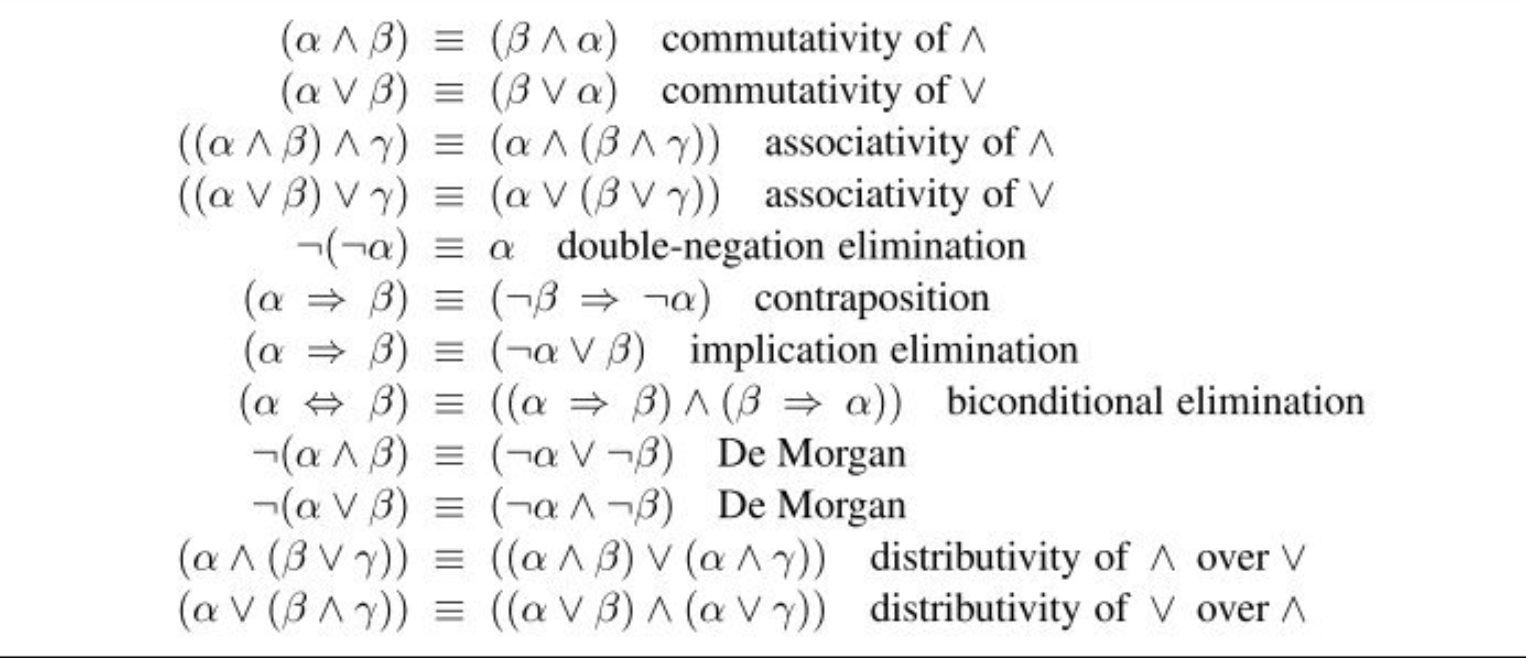
\includegraphics[width=8cm]{Standard Logical Equivalences.png}
\centering
\end{figure}

\subsubsection{Propositional Theorem Proving}

\textbf{Application of inference rules}

Legitimate (sound) generation of new sentences from old
Proof is a sequence of inference rule applications (Can use inference rules as operators in a standard search algorithm)
Typically require transformation of sentences into a normal form

\textbf{Model checking}

Truth table enumeration (always exponential in $n$)
Improved backtracking
Heuristic search in model space


\subsubsection{Propositional Inference}

There are two families of efficient algorithmns for propositional inference:
\begin{itemize}
    \item Complete backtracking search algorithms (DPLL algorithm)
    \item Incomplete local search algorithms (WalkSAT algorithm)
\end{itemize}

A statisfiability is \textbf{complete} if it terminates (returns true or false after finite time) for every sentence. An algorithm is \textbf{sound} if the returned result is correct.

Both of these algorithmns manipulate formulae in \textbf{conjunctive normal form(CNF)}

In CNF a sentence is a conjunction of clauses whose satisfiability is to be determined. A clause is a disjuntion of literals.  \newline

To convert to CNF:
\begin{enumerate}
    \item Eliminate $\Leftrightarrow$: replace $\alpha \Leftrightarrow \beta$ with $(\alpha \Rightarrow \beta)\wedge(\beta \Rightarrow \alpha)$
    \item Eliminate $\Rightarrow$: replace $\alpha \Rightarrow \beta$ with $\neg \alpha \vee \beta$
    \item Move $\neg$ inwards: use de Morgan's rules and double negation $\neg \neg a = a$
    \item Create clauses: apply distributivity law $(\vee \: over \: \wedge)$ and flatten
\end{enumerate}

The original sentence is now in CNF, as a conjunction of clauses. 

\textbf{The DPLL algorithm} determines if an input propositional logic sentence (in CNF) is satisfiable

One component of DPLL is \textbf{early termination}:
\begin{itemize}
    \item A clause is true if one of its literals is true (E.g. if A is true then $A \vee \neg B$) is true
    \item A sentence is false if any of its clauses is false (e.g. If, A is false and B is true then ($A \vee \neg B$) is false, so any sentence containing it is false)
\end{itemize}

Another aspect of DPLL is \textbf{Pure symbol heuristic}
\begin{itemize}
    \item Pure symbol: always appears with the same polarity in all clauses
    \item Make a literal containing a pure symbol true
\end{itemize}

The third component of DPLL is the \textbf{unit clause heuristic}
\begin{itemize}
    \item Unit clause: only one literal in the clause
    \item The only literal in a unit clause must be true
    \item Also includes clauses where all but one literal is false
\end{itemize}


\begin{algorithm}
\begin{algorithmic}

\Procedure{DPLL-SATISFIABLE}{$s$} 
\Comment{inputs: a sentence in propositional logic returns: true or false}
    \State $clauses \leftarrow$ the set of clauses in the CNF representation of $s$ 
    \State $symbols \leftarrow$ a list of the proposition symbols in $s$
    \State \textbf{return} DPLL($clauses,symbols,\{\}$) 
\EndProcedure \newline

\Procedure{DPLL}{$clauses,symbols,model$} \Comment{returns true or false}

    \If{every clause in $clauses$ is true in $model$} 
        \State \textbf{return} $true$
    \EndIf
    \If{some clauses in $clauses$ is false in $model$}
        \State \textbf{return} $false$
    \EndIf

    \State P,$value$ $\leftarrow$ FIND-PURE-SYMBOL($symbols,clauses,model$)
    \If{P is non-null}
        \State \textbf{return} DPLL($clauses,symbols -P, model \cup \{P=value\}$)
    \EndIf
    \State $P,value \leftarrow$ FIND-UNIT-CLAUSE($clauses,model$)
    \If{P is non-null}
        \State \textbf{return} DPLL($clauses,symbols-P,model \cup \{P = value\}$)
    \EndIf
    \State P$\leftarrow$ FIRST($symbols$); rest $\leftarrow$ REST($symbols$)

    \State \textbf{return} DPLL($clauses,rest,model \cup \{P=true\}$) or DPLL($clauses,rest,model \cup \{P=false\}$)

\EndProcedure

\end{algorithmic}
\end{algorithm}

\textbf{The WalkSat Algorithm} is an incomplete, local search algorithm. The evaluation function of WalkSat is the \textbf{min-conflict heuristic} of minimising the number of unsatisfied clauses.

The algorithm checks for satisfiability by randomly flipping the values of the variables. 

There is a balance between greediness and randomness \newline 

The below puesdocode for the algorithm takes the following inputs:
clauses, a set of clauses in propositional logic
p, the probability of choosing to do a "random walk" move, typically around 0.5
$maxFlips$, number of flips allowed before giving up \newline

And returns, a satisfying model or failure

\begin{algorithm}
\begin{algorithmic}

\Procedure{WALK-SAT}{$clauses,p,maxFlips$}
    \State $model \leftarrow$ a random assignment of $true/false$ to the symbols in $clauses$
    \For{$i = 1 \: to \: maxFlips$}

    \If{$model$ satisfies $clauses$}
        \State \textbf{return} $model$
    \EndIf

    \State $clause \leftarrow$ a randomly selected clause from $clauses$ that is false in $model$ with probability $p$ flip the value in $model$ of a randomly selected symbol from $clause$ otherwise flip whichever symbol in $clause$ maximises the number of satisfied clauses
    
    \EndFor
    \State \textbf{return} failure
\EndProcedure \newline

\end{algorithmic}
\end{algorithm}

\section{First-Order Logic}

The language of \textbf{First-order logic (FOL)}, is built around objects and relations.

FOL assumes the world contains:
\begin{itemize}
    \item Objects (people,houses,numbers,colours)
    \item Relations (red,round,prime,brother of)
    \item Functions (father of, best friend, one more than, plus)
\end{itemize}

The syntax of FOL is built on the following basic elements:
\begin{itemize}
    \item Constants (2,UoE,Richard,..)
    \item Predicates (Brother, $>$,$\leq$,...)
    \item Functions (Sqrt, LeftLegOf,...)
    \item Variables (x,y,a,b,...)
    \item Connectives ($\neg, \Rightarrow,\vee, \wedge, \Leftrightarrow$)
    \item Equality (=)
    \item Quantifiers ($\forall,\exists$)
\end{itemize}

\textbf{Atomic sentences} are formed from a predicate symbol optionally followed by a parenthesized list of terms such as $Brother(Richard,John)$. This states that Richard is the brother of John.

A term can be a function, constant or variable. \newline

An atomic sentence is true in a given model if the relation referred to by the predicate symbol holds among the objects referred to by the arguments. \newline 

\textbf{Complex formulae} are made from atomic formulae using connectives. For example, $>(1,2) \vee \leq(1,2)$ \newline

\textbf{Formulae} are mapped to an \textbf{interpretation} \newline 
An interpretation is called a model of a set of formulae when all the formulae are true for the interpretation \newline

An interpretation contains objects and relations between then. Mapping is as follows:
constant symbols $\rightarrow$ objects
predicate symbols $\rightarrow$ relation
function symbols $\rightarrow$ functions \newline 

\textbf{Universal quantification}
$\forall <variables>.<formula>$
$\forall x.P$ is true in an interpretation m if and only if P is true with x being each possible object in the interpretation. \newline

\textbf{Existential quantification}
$\exists <variables>.<formula>$
$\exists x. P$ is true for an interpretation m if and only if P is true with x being some possible object in the interpretation. Roughly speaking this is equivalent to the disjuntion of instantiations of P. \newline

\textbf{Equality}
$term_1 = term_2$ is true under a given interpretation if and only if $term_1$ and $term_2$ refer to the same object. \newline

The \textbf{deduction theorem} states that if $\alpha |= \beta$ iff $\alpha \Rightarrow \beta$ is valid

\subsection{Inference in FOL}

An inference rule for a universal instantiation (UI) is that we can infer any sentence by substituting a \textbf{ground term} for the variable i.e. $\frac{\forall v, a}{SUBST([v/g]),a}$. 

An inference rule for a existential instantiation (EI) is that we can replace the variable by a single new \textbf{constant symbol} called a \textbf{Skolem constant}. 

UI can be applied many times to produce many different outcomes while EI can be applied once, then the existentially quantified sentence could be discarded. The new knowledge base (KB) is \textbf{inferentially equivalent} to the old. Every FOL knowledge base can be propositionalised so as to preserve entailment. \newline

\textbf{Theorem:} If a sentence $\alpha$ is entailed by a FOL KB, it is entailed by a finite subset of the propositionalised KB \newline

\textbf{Theorem:} Entailment for FOL is semi-decidable i.e. algorithms exist that say yes to every entailed sentence, but no algorithm exist that also says no to every non-entailed sentence

\textbf{Modus Ponens} (Propositional Logic) is defined as $$\frac{P \: \: \: P \Rightarrow Q}{Q}$$

We can define generalised modus ponens as $$\frac{p_1', p_2',...,p_n', \: \: (p_1 \wedge p_2 \wedge ... \wedge p_n \Rightarrow q)}{SUBST(\theta, q)}$$

\subsubsection{Unification}

The goal of unification is to make different logical expressions look identical. The unify algorithm takes two sentences and returns a unifier for them if one exists $$UNIFY(p, q) = \theta$$ where $SUBST(\theta, p) = SUBST(\theta, q)$

In FOL there is a single most general unifier (MGU) that is unique up to renaming of variables. The most general unifier is the least constrained substitution that makes two clauses unify with each other. To find the MGU we can break the process down into the following steps: Decomposition, Conflict, Eliminate, Delete, Switch, Coalesce, occurs check. 

The step of decomposition is implemented as follows: \newline
Given: $$f(s_1,...,s_n) = f(t_1,...,t_n)$$, replace with $$s_1 =^? t_1,...,s_n =^? t_n$$

\subsubsection{Resolution-based Inference}

Inference procedures based on resolution work by using the principle of proof by contradiction. That is, to show that $KB |= \alpha$, we show that $KB \wedge \neg \alpha$ is unsatisfiable. 

A \textbf{definite clause} has exactly one positive literal. 

\textbf{Forward chaining} is an inference algorithm which is sound and complete for first-order definite clauses. FC may not terminate in general is $\alpha$ is not entailed. Entailment with definite clauses is semi-decidable. In incremental forward chaining there is no need to match a rule on iteration $k$ if a premise wasn't added on iteration $k-1$. \newline

\textbf{Backward chaining} is a depth-first recursive proof search in which space is linear in the size of the proof. BC is incomplete due to infinite loops. It is also inefficient due to repeated sub-goals.

\textbf{Ground Binary Resolution} is given has $$\frac{C \vee P \: \: \: \: D \vee \neg P}{C \vee D}$$. Note that if both C and D are empty then the resolution deduces the empty clause, i.e. false.  \newline

The \textbf{ground resolution theorem} is given as: If a set of clauses is unsatisfiable, then the resolution closure of those clauses contains the empty clause. 

Note that binary resolution is complete when combined with factoring. 

The \textbf{non-ground binary resolution} is given as, $$\frac{C \vee P \: \: \: \: D \vee \neg P'}{(C \vee D) \theta}$$, where $\theta$ is the mgu of P and P'. 

The Resolution algorithm takes an input a set of clauses and returns true if that set it satisfiable. It does this by performing a sequence of \textbf{resolution steps}, where each step consists of identifying two clauses of the form $c_1 = C \vee P$ and $c_2 = D \vee \not P$ and then adding $c = C \vee D$ to the \textbf{resolvent clause} \newline

The resolution algorithm will either terminate via a refutation step, or via clause saturation. When the resolvent $P \vee Q$ is the empty clause, which is logically equivalent to false we call that the refuation step and the algorithm is said to have performed a \textbf{resolution proof} (the set of clauses is unsatisfiable). 

Resolution takes two clauses and produces a new clause containing all the literals of the two original clauses except the two complementary literals. The resolution rule applies only to clauses (disjunctions of literals). 


A resolution-based theorem prover can, for any sentences $\alpha$ and $\beta$ in propositional logic, decide whether $\alpha |= \beta$ and thus resolution forms the basis for a family of complete inference procecures. 

We can summarise a resolution based algorithm as: First, ($KB \wedge \neg \alpha$) is converted into CNF.The resolution rule is applied to the CNF clauses. Each pair that contains complementary literals is resolved to produce a new clause, which is added to the set if it is not already present. The process continues until one of the two following things happens:
\begin{enumerate}
    \item There are no new clauses that can be added, in which case KB does not entail $\alpha$
    \item Two clauses reslove to yield the empty clause, in which case the KB entails $\alpha$

    
\end{enumerate}



\subsubsection{Situation Calculus}

We can introduce the notion of situations, which are logical terms. We have an initial situation and all situations generated by applying an action to a situation. We state facts about situations by relativizing predictions to situations. One can think of a situation as a sequence, or history, of actions. Two situations are only the same if their start and actions are the same

A function or relation that can vary from one situation to the next is a \textbf{fluent}. Each fluent is described with a \textbf{successor-state axiom} that says what happens to the fluent, depending on what action is taken. To describe how the world changes we can define \textbf{effect axioms} that specify the outcome of an action at the next time step. We use \textbf{frame axioms} to explicitly assert all the propositions that remain the same when an effect axiom is applied. 

In situation calculus we axiomatize all of our actions then use a general theorem prover to prove that a situation exists in which our goal is true.


\section{Symbolic Planning}

Planning is the task of coming up with a sequence of actions that will achieve a goal

In classical planning environments are:
\begin{itemize}
    \item Fully observable (accessible),
    \item Deterministic
    \item Finite
    \item Static 
    \item Discrete 
\end{itemize}

Planning Domain Definition Language or \textbf{PDDL} allows one to express many actions with one action schema.
PDDL describes:
\begin{itemize}
    \item The initial state
    \item The actions avaliable in a state
    \item The result of applying an action
    \item The goal test
\end{itemize}

Each state is represented as a conjunction of \textbf{fluents} that are ground (variable free), functionless atoms. The closed-world assumption means that any fluents that are not mentioned are false. 

The representation of states is designed so that a state can be treated either as a conjuntion of fluents, which can be manipulated by logical inference, or as a set of fluents, which can be manipulated with set operations. 


A set of ground  actions can be represented by a single \textbf{action schema}. The schema is a lifted representation - it lifts the level of reasoning from propositional logic to a restricted subset of first-order logic. A schema consists of the action name, a list of all the variables used in the schema, a precondition and an effect. The variables should be thought of as being universally quantified. 

$$(a \in ACTIONS(s)) \leftrightarrow (s \vDash PRECOND(a))$$

We say that action $a$ is \textbf{applicable} in state $s$ if the preconditions are satisfied by $s$. \newline

Basic PDDL does not allow quantifiers. 

\subsection{State-space search}

State-space search searches the space of states using action schemata. There are two methods of doing this.

\begin{itemize}
    \item Forward state-space search - start in initial state and consider action sequences until goal state is reached
    \item Backward state-space search - Start from goal state; consider action sequences until initial state is reached
\end{itemize}

\textbf{Heuristics for state space search} can be:
\begin{itemize}
    \item Divide and Conquer (subgoal decomposition)
    \item Derive a Relaxed problem
\end{itemize}

Subgoal decomposition is:
\begin{itemize}
    \item Optimistic if negative interactions exist (subplan deletes goal achieved by other subplan)
    \item Pessimistic if positive interactions exist (subplans contain redundant actions)
\end{itemize}

Relaxations:
\begin{itemize}
    \item Drop all preconditions (all actions always applicable, combined with subgoal independence makes prediciton even easier)
    \item Remove all negative effects (and count minimum number of action so that union satisfies goals)
    \item Empty delete lists approach (involves running a simple planning problem to compute heuristic value)
\end{itemize}

\subsection{Partial-order planning}

The basic idea of partial order planning is to add actions to a plan without specifying which comes first unless necessary and next combine 'independent' sub-sequences afterwards. The partial-order solution will correspond to one or several linearisations of partial-order plan. Search in plan space rather than state spaces. 

Partial order planning can be defined as a search problem over plans consisting of:
\begin{itemize}
    \item Actions; initial plan contains dummy actions Start (no preconditions, effect  = initial state) and Finish (no effects, precondition = goal literals)
    \item Ordering constraints on actions A $\prec$ B (A must occur before B); contradictory constraints prohibited 
    \item Causal links between actions A $\rightarrow^p $ B express A achieves p for B (p precondition of B, effect of A, must remain true between A and B); inserting action C with effect $\neg p$ (A $\prec$ C and C $\prec$ B) would lead to conflict.
    \item Open preconditions: set of conditions not yet achieved by the plan (planners try to make open precondition set empty without introducing contradictions)
\end{itemize}

A \textbf{consistent plan} is one without cycles in orderings and conflicts with links and a \textbf{solution} is a consistent plan without open preconditions. 

The partial-order planning algorithm is as follows:
\begin{itemize}
    \item Inital plan: Actions: {Start, Finish}, orderings: {Start $\prec$ Finish},
          Links: {}, Open preconditions: Preconditions of Finish
    \item Pick p from open preconditions on some action B, generate a consistent successor plan for every A that achieves p
    \item Ensuring consistency:
            Add A$\rightarrow^p$ B and A $\prec$ B to plan. If A new, add A and Start $\prec$ A and A $\prec$ Finish to plan
            Resolve conflicts between the new link and all actions and between A (if new) and all links as follows: If conflict between A $\rightarrow^p$ B and C, add B $\prec$ C or C $\prec$ A
    \item Goal test: check whether there are open preconditions
\end{itemize}



\subsection{Planning and acting in the Real World}


Methods for handling indeterminacy include:

\textbf{Sensorless/conformant} planning: achieve goal in all possible circumstances, relies on coercion. \textbf{Contingency} planning: for partially observable and bounded non-deterministic environments; includes sensing actions and describes different paths for different circumstances. \textbf{Online planning and replanning}: check whether plan requires revision during execution and replan accordingly

\subsubsection{Partially observable environments}

In partially observable environments we can allow variables in preconditions that aren't part of the action's variable list.

A \textbf{percept schema} models that agent's sensors; it tells the agent what it knows, given certain conditions about the state it's in. 

A fully observable environment has a percept axiom for each fluent with no preconditions. A sensorless planner has no percept schemata at all.

When one doesn't know the value of all relevant fluents they must plan using beliefs. When actions have more than one outcome one needs to represent the conditional effects in action schemata.

A \textbf{belief state} corresponds exactly to the set of possible worlds that satisfy the formula - open world assumption. 

In sensor-less planning you can only apply actions whose preconditions are satisfied by your current belief state $b$

The update of a belief state $b$ given an action $a$ is the set of all states that result from doing $a$ in each possible state $s$ that satisfied belief state $b$


 \subsubsection{Execution monitoring and replanning}

\textbf{Unbounded non-determinancy} Is a situation where you have actions that have an unbounded number of possible consequences. 

 \textbf{Execution monitoring} is the process of checking whether things are going according to plan. 
 \textbf{Action monitoring} is the process of checking whether the next action is feasible 
 \textbf{Plan monitoring} is the process of checking whether the remainder of plan is feasible. 

 \textbf{Re-planning} is the ability to find new plan when things go wrong.

 \subsubsection{Hierarchical Planning}

 \textbf{Hierarchical planning} is a problem-solving approach that involves breaking down complex tasks into a hierarchical structure of smaller sub-tasks or actions that can be executed by an intelligent agent.

At each level of the hierarchy, activity involves only small number of steps

\textbf{Hierarchical task network planning}: Initial plan provides only a high-level description ,refined by action refinements. 

Refinement process is continued until the plan consists only of primitive actions. Primitive actions are action that one can execute

\textbf{High-Level plans} (HLP) are a sequence of high-level actions (HLA), with an implementation of a High Level Plan being the concatenation of an implementation of each of its HLAs.

A HLP achieves the goal from its initial state if at least of its implementations does this. Not all implementations of an HLP have to reach the goal state. 

\textbf{Searching for primitive solutions: Breadth First} \newline

\begin{itemize}
    \item Start your plan (HLP) with the HLA [Act]
    \item Take the first HLA A in P (P is an action sequence)
    \item Do breadth-first search in your hierarchical plan library, to find a refinement of A whose preconditions are satisfied by the outcome of the action in P that is prior to A. 
    \item Replace A in P with this refinement
    \item Keep going until your plan has no HLAs and either: (1) Your plan P's outcome is the goal, in which case return P or (2) your plan P's outcome is no the goal in which case backtrack and if nowhere to backtrack true then return failure
\end{itemize}

There are issues with this approach:
\begin{itemize}
    \item Lots of irrelevant actions are considered
    \item The algorithm essentially refines HLAs right down to primitive actions so as to determine of a plan will succeed
\end{itemize}

One challenge in specifying preconditions and effects of an HLA is that the HLA may have more than one refinement, each one with slightly different preconditions and effects. 

$s' \in Reach(s,h)$ if and only if $s'$ is reachable from at least one of the HLA h's refinements, given initial state s. 

HLP p achieves goal g given initial state $s$ if and only if $\exists s'$ such that $s' |= g$ and $s' \in Reach (s, p)$ \$

Thus, we should search HLPs to find a $p$ with this relation to $g$ and then focus on refining it. But a pre-requisite to this algorithm is to define Reach(s,h) for each $h$ and $s$

A \textbf{primitive action} makes a fluent true, false, or leaves it unchanged. However, with HLAs you sometimes get to choose, by choosing a particular refinement. \newline

An Optimistic Description of which states are reachable given a HLA: $Reach^+(s,h)$
\begin{itemize}
    \item Take union of all possible outcomes from all refinements
    \item This overgenerates reachable states
\end{itemize}

Pessimistic description of what is reachable: $Reach^-(s,h)$
\begin{itemize}
    \item Only states that satisfy effects from all refinements survive
    \item This undergenerates reachable states
\end{itemize}

Notes:
\begin{enumerate}

    \item If there is a state $s'$ such that $s' |= g$ in the pessimistic description of what is reachable, you know $h$ can succeed 
    \item If there does not exist a state $s'$ in the optimistic description of what is reachable you know $h$ will fail

    
\end{enumerate}

Thus we define an algorithm for finding a plan as:
\begin{itemize}
    \item Do breadth first search as before
    \item Stop searching and implement instead when you reach an $h$ where 1. is true
    \item You can drop $h$ (and all of its refinements) when 2. is true
    \item If 1. and 2. are both false for the current $h$ then you don't know if $h$ will succeed or fail, but you can find out by refining it
\end{itemize}

\section{Acting under uncertainty}

\subsection{Rational decisions}

A logical agent has a goal and executes any plan guaranteed to achieve it. This is different with degrees of belief in which case an agent must have preferences over outcomes of plans. Utility theory can be used to reason about those preferences. Agents must balance the trade-off between cost and utility. Based on the idea that every state has a degree of usefulness and agents prefer states with higher utility. Utilities vary from one agent to another.

Decision theory combines probability theory and utility theory. The foundation of decision theory is: "An agent is rational if and only if it chooses the action that yields the highest expected utility, averaged over all possible outcomes of the action".

\subsection{Probability Theory}

An atomic event is a complete specification of the state of the world. Atomic events are mutually exclusive. The set of atomic events is exhaustive. Every event entails the truth or falsehood of any proposition. 

A probability distribution is the probabilities of all values of a random variable. 

A joint probability distribution is the cross-product of individual distributions.

$P(A|B) = \frac{P(a \wedge b)}{P(b)}$
$P(x_1, \ldots, x_n) = \Pi_{i=1}^n P(x_i | x_{i-1},\ldots, x_1)$

\subsection{Probabilistic Inference}

\subsubsection{Joint Probability Distributions}

Extracting distribution of subset of variables is called \textbf{marginalisation} $$P(Y) = \sum_z P(Y, z)$$

We can derive the following definition of marginalisation by using the product rule: $$P(Y) = \sum_z P(Y|z)P(z)$$

Normalisation ensures probabilities sum to 1, normalisation constants are often denoted by $\alpha$

We can conduct a general inference procedure where we let: X be a query variable, E set of evidence variables and $e$ their observed values, Y the remaining unobserved variables. 

Query evaluation is computed as: $P(X|e) = \alpha P(X, e) = \alpha \sum_y P(X)$

Note that X, E and Y constitute the complete set of variables

\subsubsection{Independents and Bayes' Rule}

A variable X is \textbf{independent} of a variable Y if $P(X|Y)$ is equal to $P(X)$ similarly $P(Y|X) = P(Y)$ also $P(X,Y) = P(X)P(Y)$ 

Independence assumptions can help to dramatically reduce complexity. 

\textbf{Bayes' rule} is derived by writing the product rule in two forms and equating them, yielding 

$$P(b|a) = \frac{P(a|b)P(b)}{P(a)}$$

The general case for multi-varied variables using background evidence $e$: $$P(Y|X,e) = \frac{P(X|Y,e)P(Y|e)}{P(X|e)}$$

Two variables X and Y are conditionally independent given Z if $P(X,Y|Z) = P(X|Z)P(Y|Z)$, this is equivalent to $P(X|Y,Z) = P(X|Z), P(Y|X,Z) = P(Y|Z)$

\subsection{Bayesian Networks}

Bayesian Networks are graphs consisting of nodes representing random variables which are connected whenever they depend on each other. Intuitively, links describe \textbf{direct effects} of variables on each other in the domain. We can assume anything that is not directly connected does not dircetly depend on each other. \newline

Formally:

A Bayesian network is a directed acyclic graph with nodes annotated with probability information. Nodes represent random variables (discrete or continuous). Links connect nodes, if there is an arrow from X to Y one calls X a parent of Y. Each node $X_i$ has a conditional probability distribution (CPD) attached to it. The CPD describes how $X_i$, depends on its parents, its entries describe $P(X_i | Parent(X_i))$. \newline

Each variable is conditionally independent of its non-descendants, given its parents: If $X \notin Parents*(Y)$, then $$P(X| Parents(X),Y) = P(X | Parents(X))$$ \newline

$P(x_1, \ldots, x_n) = \Pi_{i=1}^n P(x_i, parents(X_i))$

Note: Ensure you start at the bottom of the graph. \newline

Topological semantics:
\begin{enumerate}
    \item A node is conditionally independent of its non-descendants given its parents
    \item A node is conditionally independent of all other nodes, given its parents, children and children's parents, this is defined as its \textbf{Markov blanket}
\end{enumerate}

\textbf{Noisy-OR} relationships: \newline

Any cause can make effect true, but won't \textit{necessarily} (effect inhibited; $P(effect | cause) < 1$)

Noisy-OR assumes inhibitions are mutually conditionally independent and that all causes are listed (\textbf{leak node} can be used to catch miscellaneous unlisted causes)

Whatever inhibits $C_1$ from making E true is independent of what inhibits $C_2$ from making E true.

Hence E is false if and only if each of its true parents are inhibited and we can compute this likelihood from the product of probabilities for each individual cause inhibiting E. \newline

\textbf{BNs with continuous variables} \newline

We can use standard families of probability distributions defined in terms of a few parameters such as a normal distribution. 

Hybrid BNs use a mixture of discrete continuous variables.

\subsubsection{Exact Inference in Baysian networks}

Informally inference is the task of computing a posterior distribution for a set of query variables given some observed event. \newline

Formally: Determine $P(X|e)$ given query variables X, evidence variables, E (and non-evidence or hidden variables Y) \newline

\textbf{Inference by enumeration:}

$$P(X | E) = \frac{P(X, E)}{P(E)} = a P (X, E) = a \sum_{y \in Y} P(X, E, y)$$ 

We then construct a tree of the operations moving left to right after removing terms that do not depend on the sum variables.

\textbf{Variable elimination}

The idea of variable elimination is to avoid the repeated calculations found in enumeration, with the basic idea being to store results after doing a calculation once. This method works bottom-up by evaluating sub expressions.

To do this we annotate each part of the expression with a factor. A factor is a matrix, indexed with its argument variables.

We evaluative the new expression containing the factors via point wise product. When we sum out each expression we are left with a new factor. 

Point-wise product yields the product for the union of variables in its arguments.

We can eliminate all variables that aren't ancestors of query or evidence variables.

\subsection{Approximate Inference Methods}

Since exact inference is computationally very hard, we use approximate methods such as randomised sampling algorithms

\subsubsection{Direct Sampling Methods in BNs}

The goal of direct sampling is to generate samples from a known probability distribution. The simplest method of direct sample is to generate events from network without evidence, in a Bayes network we can sample each variable in 'topological order'. 

This technique generates samples with probability $S(x_1, \ldots, x_n)$ yielding, $$S(x_1, \ldots, x_n) = P(x_1, \ldots, x_n) = \Pi_{i=1}^n P(x_i | parents(X_i))$$. 

Answers are computed by counting the number $N(x_1, \ldots, x_n)$ of times the event $x_1, \ldots, x_n$ was generated and dividing by total number $N$ of all samples.

In the limit, we should get $$\lim_{n \to \infty} \frac{N(x_1, \ldots, x_n)}{N} = P(x_1, \ldots, x_n)$$

If the estimated probability becomes exact in the limit we call the estimate consistent \newline

\textbf{Rejection sampling} \newline

The purpose of rejection sampling to to produce samples for hard-to-sample distribution from easy-to-sample distribution. To determine $P(X|e)$ one should generate samples from the prior distribution specified by the BN first, then we reject those that do not match the evidence. 

The estimate $\hat{P} (X = x|e)$ is obtained by counting how often $X = x$ occurs in the remaining samples.

Rejection sampling is consistent because by definition: $$\hat{P} (X|e) = \frac{N(X, e)}{N(e)} = \frac{P(x, e)}{P(e)} = P(X|e)$$ 

\textbf{Likelihood Weighting} \newline

This is a direct sampling method that avoids inefficiency of rejection sampling by generating only samples consistent with evidence. This method fixes the values for evidence variables $E$ and samples only the remaining variables $X$ and $Y$. \newline

Since not all events are equally probable, each event has to be weighted by its likelihood that it accords to the evidence. Likelihood is measured by product of conditional probabilities for each evidence variable, given its parents. 

 $S(z,e) = = \Pi_{i=1}^I P(z_i | parents(Z_i))$

 S's sample values for each $Z_i$ is influenced by the evidence among $Z_i$'s ancestors. S pays no attention when sampling $Z_i$'s value to evidence from $Z_i$'s non-ancestors; so not sampling from the true posterior probability distribution.

The likelihood weight $w$ makes up for the difference between the actual and desired sampling distributions: 

$$w(z,e) = \Pi_{i=1}^m P(e_i | parents(E_i))$$

Since two products cover all the variables in the network, we can write: $$P(z,e) = \Pi_{i=1}^I P(z_i |parents(Z_i))\Pi_{i=1}^m(e_i | parents(E_i))$$

We can observe that likelihood weighting is consistent. However most samples will have very small weights as the number of evidence variables increases. 

\textbf{The Markov chain Monte Carlo (MCMC) algorithm} 

The basic idea behind the MCMC algorithm is to create an event from a previous event, rather than generate all events from scratch. One can view the BN as having a current state specifying a value for each variable. Consecutive state is generated by sampling a value for one of the non-evidence variables $X_i$ conditioned on the current values of variables in the Markov blanket of $X_i$. The algorithm randomly wanders around the state space flipping one variable at a time and keeping evidence variables fixed. \newline

An informal proof that MCMC is consistent: The sampling process settles into a "dynamic equilibrium" in which the long-term fraction of time spent in each state is exactly proportional to its posterior probability. 

\subsection{Time and Uncertainty}

In dynamic processes we can imagine one BN model of the problem for every time step and reason about changes between them. 

\subsubsection{Stationary Processes}

Series of time slices will be used to describe processes of change. Time slices consist of observable random variables $E_t$ and non-observable ones $X_t$. We assume sets of (non) observable variables remain constant over time, but this is not necessary. Observation at will be $E_t = e_t$ for some set of values $e_t$. We assume that states start at $t=0$ and evidence starts arriving at $t=1$.

Note: We use the notation $a:b$ to denote sequences of integers e.g $U_1, U_2, U_3$ = $U_{1:3}$

We assume that changes are caused by a \textbf{stationary process} - the laws that govern change do not change over time. E.g. $P(U_t | Parents(U_t))$ does not depend on $t$. 

\subsubsection{Markov Assumption}

To ensure we do not have an unbounded number of parents in the set of variables we use the Markov assumption. The \textbf{Markov assumption} defines that the current state only depends on a finite history of previous states. In a first-order Markov process every state depends only on predecessor state. Under the first-order Markov assumption we can write the transition model as $$P(X_t | X_{0:t-1}) = P(X_t | X_{t-1})$$

We assume that evidence variables are conditionally independent of other stuff given the current state, referred to as the \textbf{sensor model} of the system: $$P(E_t | X_{0:t}, E_{0:t-1}) = P(E_t | X_t)$$. 

In the sensor model the state causes evidence. \newline

The prior distribution over initial states is denoted as $P(X_0)$ \newline

Using the three distribution we yield the complete joint probability distribution: $$P(X_0, X_1, \ldots, E_1, \ldots, E_t) = P(X_0)\Pi_{i=1}^t P(X_i, X_{i-1})P(E_i | X_i)$$ \newline

\subsubsection{Inference in Temporal Models}

One type of inference task in a temporal model is \textbf{filtering/monitoring} in which we compute a \textbf{belief state} given the evidence to date i.e. $P(X_t | e_{1:t})$. 
Another is \textbf{prediction} in which we compute a posterior distribution over a future state given the evidence to date i.e. $P(X_{t+k} | e_{1:t})$. \newline

Filtering is done by recursive estimation i.e. we compute the result for $t+1$ by doing it for $t$ and then updating with new evidence $e_{t+1}$ That is, for some function f: $$P(X_{t+1} | e_{1:t+1}) = f(e_{t+1}, P(X_t | e_{1:t}))$$, from this expression we derive: $$\alpha' P(e_{t+1} | X_{t+1})\sum_{x_t} P(X_{t+1} | x_t) P(x_t | e_{1:t})$$

Prediction works like filtering without new evidence. Computation involves only the transition model and not the sensor model. $$P(X_{t+k+1} | e_{1:t}) = \sum_{x_{t+1}} P(X_{t+k+1} | x_{t+k})P(x_{t+k}|e_{1:t})$$ \

\textbf{Smoothing(Hindsight)}

Smoothing is the computation of a distribution of past states given current evidence i.e. $P(X_k | e_{1:t}), 1 \leq k < t$

We can view this as a 2-step process going up to $k$ and then $k+1$ to $t$ \newline

$P(X_k | e_{1:t}) = P(X_k | e_{1:k}, e_{k+1:t})$ from which we derive $$P(X_k | e_{1:t}) = \alpha f_{1:k}b_{k+1:t}$$

\textbf{Best Explanation and HMMs}

To find the most likely sequence there is a recursive relationship between the most likely paths to $x_{t+1}$ and the most likely paths to each state $x_t$ $$max_{x_1,...,x_t} P(x_1,...,x_t, X_{t+1} | e_{1:t+1})$$

This algorithm (Viterbi algorithm) runs forward along sequence computing $m$ message in each step. In the end this has the probability for the most likely sequence for reaching each final state and thus it is easy to determine the overall most likely sequence. 

\textbf{Hidden Markov Models (HMMs)} are defined as a temporal probabilistic model in which the process is described by a single variable. The structure of HMMs allows for a very simple matrix implementation of basic algorithms. 

 \subsection{Rational Decision Making}

 \subsubsection{Dynamic Bayesian Networks}

A Dynamic Bayesian Network (DBN) is a BN describing a temporal probability model that can have any number of state variables $X_t$ and evidence variables $E_t$. HMMs are DBNs with a single state and a single evidence variable.

To construct a DBN we have to specify prior distribution of state variables $P(X_0)$, transition model $P(X_{t+1} | X_t)$, and sensor model $P(E_t | X_t)$. 

Transient failure occurs when a sensor occasionally sends inaccurate data. 

Persistent failure models describe how a sensor behaves under normal conditions and after failure.

\subsubsection{Preferences and Uncertainty}

Rational agents do things that are an optimal trade off between: the likelihood of reaching a particular resultant state and the desirability of that state. 

Agents preferences between wold states are described using a utility function. A utility function assigns some numerical value $U(S)$ to each state $S$ to express its desirability for the agent. Nondeterministic action $a$ has results $Result(a)$ and probabilities $P(Result(a) = s'|a,e)$ summarise the agent's knowledge about its effects given evidence observations $e$ We can thus obtain the expected utility (EU) as $$EU(A|E) = \sum_{s'}P(\text{Result(a) = } s'|a,e)U(s')$$

The principle of \textbf{maximum expected utility (MEU)} says that an agent should use the action that maximises expected utility. 

Rational preferences have the following constraints:
\begin{itemize}
    \item Continuity: If B is between A and C in preference, then with some probability the agent will be indifferent between getting B for sure and a lottery over A and C
    \item Substituability: indifference between between lotteries leads to indifference between complex lotteries built from them
    \item Monotonicity Preferring A to B implies preference for any lottery that assigns a higher probability to A
    \item Orderability 
    Transitivity: If an agent prefers A over B and B over C then they must prefer A over C
    \item Decomposability: Compound lotteries can be reduced to a simpler one
\end{itemize}

\subsubsection{Decision Networks}

\textbf{Decision networks} combine BNs with additional node types for actions and utilities. 

In a DN \textbf{chance nodes} (ovals) represent random variables with CPTs, parents can be decision nodes. \textbf{Decision nodes} represent decision making points at which actions are available. \textbf{Utility nodes} represent the utility function connected to all nodes that affect utility directly. Often nodes describing outcome states are omitted and expected utility associated with actions is expressed in \textbf{action-utility tables}

Evaluation of a DN works by setting decision node to every possible value

The algorithm is given as:
\begin{itemize}
    \item Set evidence variables for current state
    \item For each value of decision node: Set the decision node to that value, calculate the posterior probabilities for parents of utility node and then calculate the resulting utility for the action
    \item Return action with the highest (expected) utility
\end{itemize}

\subsection{Markov Decision Processes}

A \textbf{transition model} $T(s,a,s')$ denotes the probability that action $a$ in $s$ will lead to state $s'$. A \textbf{Markovian} model, is one in which the probability of reaching $s'$ depends only on $s$ and not on history of earlier states. \newline

A \textbf{Markov Decision Process (MDP)} has an initial state $S_0$, transition model $T(s,a,s')$ and a utility function. The solution solution should describe what the agent does in every state, this is called \textbf{policy}, denoted as $\pi$. $\pi(s)$ for an individual state describes which action should be taken in $s$. An \textbf{optimal policy} is one that yields the highest expected utility, denoted by $\pi*$ \newline

A \textbf{finite horizon} means there is a fixed time $N$ after which nothing matters. 

\subsubsection{Computing optimal policies}

For a finite horizon we have non-stationary optimal policies ($N matters$). However, with an infinite horizon we get \textbf{stationary} optimal policies. For \textbf{additive rewards} we get $$U_h(s_0, s_1, s_2, ...) = R(S_0) + R(S_1) + R(S_2) + ...$$. For \textbf{discounted rewards}, we use a discount factor $0 \leq \gamma \leq 1$ to yield $$U_h(s_0,s_1,s_2,...) = R(s_0) + \gamma R(S_1) + \gamma^2 R(S_2) + ...$$. This discount factor makes more distant future rewards less significant. 

\textbf{Value iteration} is an algorithm for calculating optimal policy in MDPs in this we calculate the utility of each state and then select the optimal action based on these utilities. 

The criterion for optimal policy with discounted is given as $$\pi^* = argmax_{\pi} E (\sum_{t=1}^{\infty} \gamma^t R(s_t)|\pi)$$ 

Given $U(s)$, we can easily determine an optimal policy: $\pi^* (s) = argmax_{a} \sum_{s'} T(s,a,s')U(s')$. The utility of a state is immediate reward plus expected utility of subsequent states is agent chooses an optimal action. The \textbf{Bellman} equation can be defined as $$U(s) = R(s) + \gamma max_{a} \sum_{s'} T(s,a,s')U(s')$$

The value iteration algorithm is given as follows: For $n$ states we have $n$ Bellman equations with $n$ unknowns, value iteration is an iterative approach to solving the $n$ equations. We start with arbitrary values and update them as follows: $$U_{i+1} \leftarrow R(s) + \gamma max_a \sum T(s,a,s')U_i (s')$$

This algorithm converges to a right and unique solution. 

\end{document}